\begingroup\hyphenpenalty=10000\relax
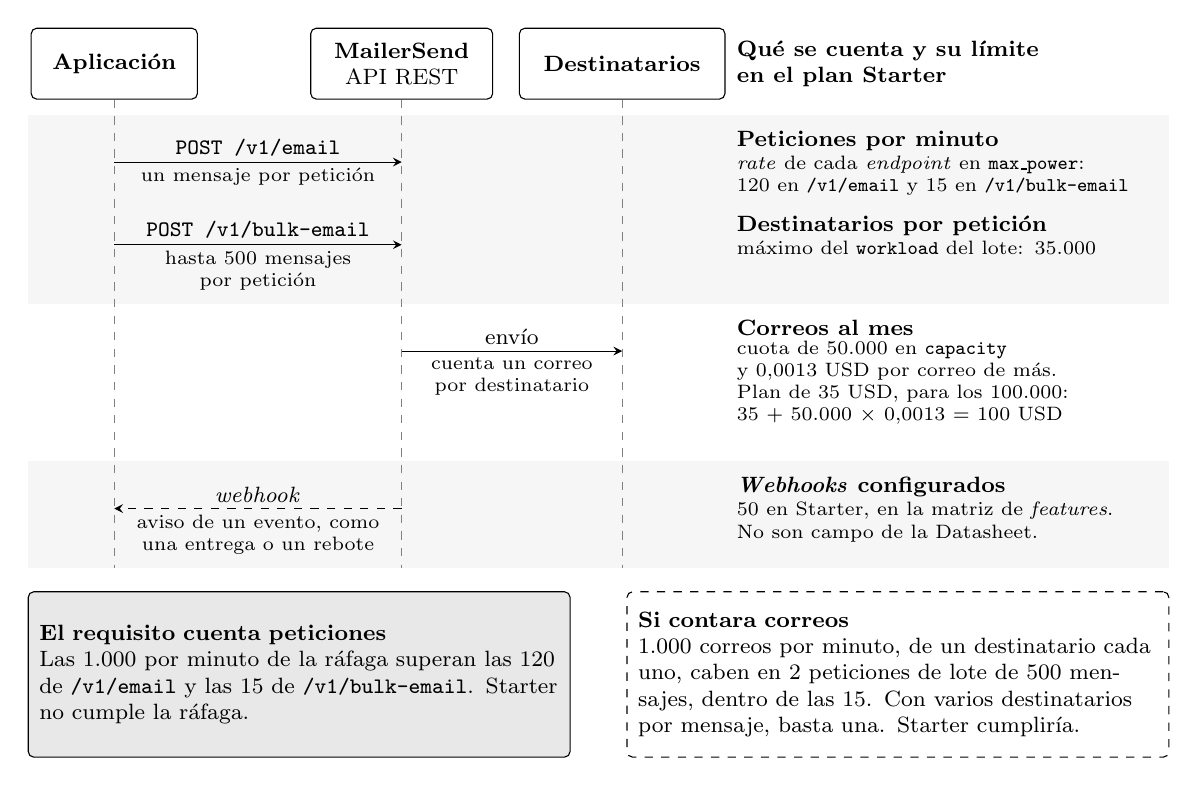
\begin{tikzpicture}[
  font=\footnotesize,
  actor/.style={draw, rounded corners=2pt, align=center, minimum height=9mm, inner sep=3pt},
  cabecera/.style={font=\footnotesize\bfseries, align=left, anchor=west, inner sep=0pt},
  arriba/.style={font=\footnotesize, anchor=south, inner sep=2pt},
  abajo/.style={font=\scriptsize, align=center, anchor=north, inner sep=2pt},
  unidad/.style={font=\footnotesize\bfseries, align=left, text width=55mm, anchor=north west, inner sep=0pt},
  limite/.style={font=\scriptsize, align=left, text width=55mm, anchor=north west, inner xsep=0pt, inner ysep=1.5pt},
  lectura/.style={draw, rounded corners=2pt, align=left, text width=66mm, minimum height=21mm, inner sep=4pt}
]
\fill[gray!7] (0,-1.15) rectangle (14.5,-3.55);
\fill[gray!7] (0,-5.55) rectangle (14.5,-6.9);
\node[actor, text width=19mm] (app) at (1.1,-0.5) {\textbf{Aplicación}};
\node[actor, text width=21mm] (api) at (4.75,-0.5) {\textbf{MailerSend}\\ API REST};
\node[actor, text width=24mm] (dest) at (7.55,-0.5) {\textbf{Destinatarios}};
\node[cabecera, text width=55mm] at (9.0,-0.5) {Qué se cuenta y su límite\\ en el plan Starter};
\draw[dashed, gray] (app.south) -- (1.1,-6.9);
\draw[dashed, gray] (api.south) -- (4.75,-6.9);
\draw[dashed, gray] (dest.south) -- (7.55,-6.9);
\draw[-stealth] (1.1,-1.75) -- node[arriba] {\texttt{POST /v1/email}} node[abajo] {un mensaje por petición} (4.75,-1.75);
\draw[-stealth] (1.1,-2.8) -- node[arriba] {\texttt{POST /v1/bulk-email}} node[abajo] {hasta 500 mensajes\\ por petición} (4.75,-2.8);
\node[unidad] (u1) at (9.0,-1.35) {Peticiones por minuto};
\node[limite] (l1) at (u1.south west) {\textit{rate} de cada \textit{endpoint} en \texttt{max\_power}:\\ 120 en \texttt{/v1/email} y 15 en \texttt{/v1/bulk-email}};
\node[unidad] (u2) at ([yshift=-2mm]l1.south west) {Destinatarios por petición};
\node[limite] at (u2.south west) {máximo del \texttt{workload} del lote: 35.000};
\draw[-stealth] (4.75,-4.15) -- node[arriba] {envío} node[abajo] {cuenta un correo\\ por destinatario} (7.55,-4.15);
\node[unidad] (u3) at (9.0,-3.75) {Correos al mes};
\node[limite] at (u3.south west) {cuota de 50.000 en \texttt{capacity}\\ y 0,0013 USD por correo de más.\\ Plan de 35 USD, para los 100.000:\\ 35 + 50.000 $\times$ 0,0013 = 100 USD};
\draw[-stealth, dashed] (4.75,-6.15) -- node[arriba] {\textit{webhook}} node[abajo] {aviso de un evento, como\\ una entrega o un rebote} (1.1,-6.15);
\node[unidad] (u4) at (9.0,-5.75) {\textit{Webhooks} configurados};
\node[limite] at (u4.south west) {50 en Starter, en la matriz de \textit{features}.\\ No son campo de la Datasheet.};
\node[lectura, fill=gray!18, anchor=north west] at (0,-7.2) {\textbf{El requisito cuenta peticiones}\\ Las 1.000 por minuto de la ráfaga superan las 120 de \texttt{/v1/email} y las 15 de \texttt{/v1/bulk-email}. Starter no cumple la ráfaga.};
\node[lectura, dashed, anchor=north east] at (14.5,-7.2) {\textbf{Si contara correos}\\ 1.000 correos por minuto, de un destinatario cada uno, caben en 2 peticiones de lote de 500 mensajes, dentro de las 15. Con varios destinatarios por mensaje, basta una. Starter cumpliría.};
\end{tikzpicture}
\endgroup
